\section{Overview of Natural Language Processing}
Natural Language Processing (NLP) as a field covers a wide range of tasks that all relate around the concept of creating models of either some aspect of language or more ambitiously all aspects of language. These models are then normally used to create structure for the vast quantities of text that contains no structure at all. NLP tasks can be categorised based on the linguistics property the tasks are solving e.g. syntactic or semantic task, of which these properties and thus the tasks are generally hierarchical. The low level syntactic tasks tend to be sequence labelling problems for instance Part Of Speech (POS) tagging \citep{church-1988-stochastic, ling-etal-2015-finding} or Chunking \citep{tjong-kim-sang-buchholz-2000-introduction}. The low level syntactic information is usually used to guide the higher level syntactic tasks such as dependency \citep{nivre-etal-2007-conll} and constituency parsing \citep{collins-2003-head}. As can be seen from the constituency and dependency trees within figure \ref{fig:lit_review_constituency_tree}\footnote{Constituency tree demo URL \url{https://demo.allennlp.org/constituency-parsing}} and \ref{fig:lit_review_dependency_parse_tree}\footnote{Dependency tree demo URL \url{https://demo.allennlp.org/dependency-parsing}} the POS tags correlate largely with the constituency and dependency labels e.g. a noun (\textit{NN}\footnote{Singular noun.}) being part of a noun phrase (\textit{NP}) and a noun (\textit{NNS}\footnote{Plural noun.} or \textit{NN}) being the modifier in the nominal subject modifier (\textit{NSUBJ}). The relation between lower and higher level syntactic tasks has been explicitly shown to be hierarchical within \citet{sogaard-goldberg-2016-deep} multi task learning work. The relation between tasks extends beyond the categories where syntactic information is useful within semantic based tasks, for instance within text classification. The example sentence within the figures is a neutral sentence as it contains an equal amount of positive and negative sentiment\footnote{If the sentence is put through Stanford CoreNLP 3.9.2 it would also classify the sentence as neutral. URL to Stanford CoreNLP 3.9.2 \url{https://corenlp.run/}}. To know the sentiment of the sentence it requires knowing that words such as \textit{great} are positive words, semantic knowledge. Further for the example sentence knowing that the words \textit{was n't} modifies the meaning of the word \textit{great} requires syntactic (from the dependency tree, figure \ref{fig:lit_review_dependency_parse_tree}) and semantic information. Similar to the syntactic tasks, semantic tasks also have a hierarchical structure where some tasks require less language understanding than others \citet{sanh2019hierarchical}. For a more comprehensive overview of syntactic and semantic tasks in NLP and how they relate see Chapter 6 and 7 in \citet{goldberg2017neural}. In recent years it has been shown that utilising NN that have been initially trained on a high level NLP tasks such as Masked Language Modelling (MLM) \citep{devlin-etal-2019-bert} can be useful for the whole NLP pipeline (syntactic to semantic tasks) \citep{tenney-etal-2019-bert}. Thus finally showing how the tasks are hierarchical in nature. This brief primer into NLP does not touch on any topics that utilises NLP with any other modality, such as images for image captioning \citep{Karpathy_2015_CVPR}, audio for sentiment analysis \citep{raaijmakers-etal-2008-multimodal}, and many more.

%training on very high level semantic tasks such as Language Modelling and Machine Translation can 

%Lastly to 
%In recent years it has been shown that language modelling has been the most universal NLP task that has significant impact on improving the performance on other NLP task no matter if they are semantic or syntactic. Thus showing that training models on


%To further iterate the point on how the tasks are hierarchical, \citet{sogaard-goldberg-2016-deep} found that using POS tagging as an auxiliary task at the first layer of a multi layer Neural Network (NN) to be beneficial to multiple higher level syntactic tasks that are predicted at the top layer of the NN. \citet{sanh2019hierarchical} found the same for semantic tasks where treating them in a hierarchy can help tasks at all levels of the semantic hierarchy.  

%syntactic information is useful to semantic task and within a hierarchical framework 

%These tasks can be seen as hierarchical in nature where knowing how to perform one task can help and/or influence another task. The tasks can range from 


\begin{figure}[!h]
    \centering
    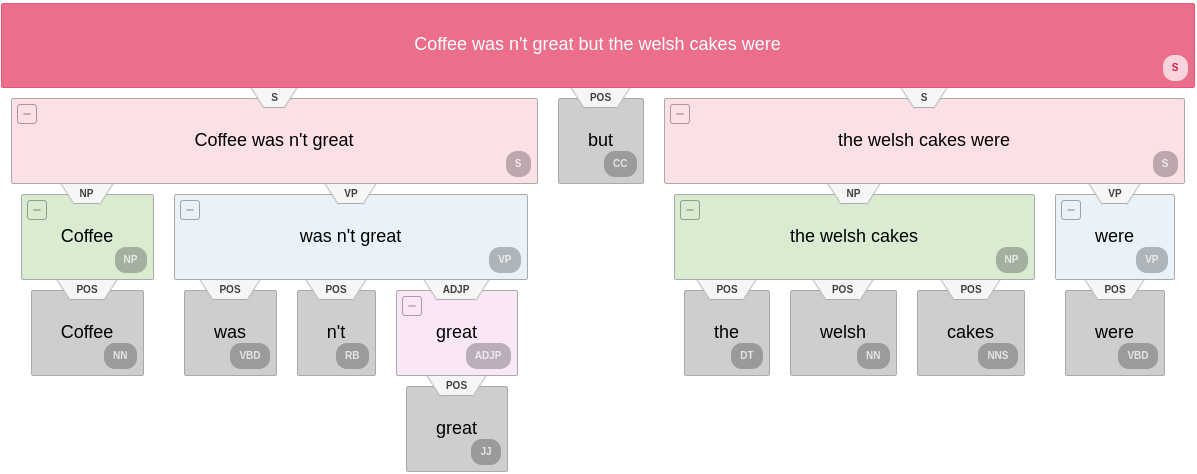
\includegraphics[scale=0.28]{images/lit_review/constituency_tree.png}
    \caption{Constituency tree for the sentence `Coffee wasn't great but the welsh cakes were'. The labels in each box represents the constituency label for that span, the labels for the leaf nodes are the POS tags for those words. The tree was created using the AllenNLP demo, which used \citet{joshi-etal-2018-extending} model.}
    \label{fig:lit_review_constituency_tree}
\end{figure}

\begin{figure}[!h]
    \centering
    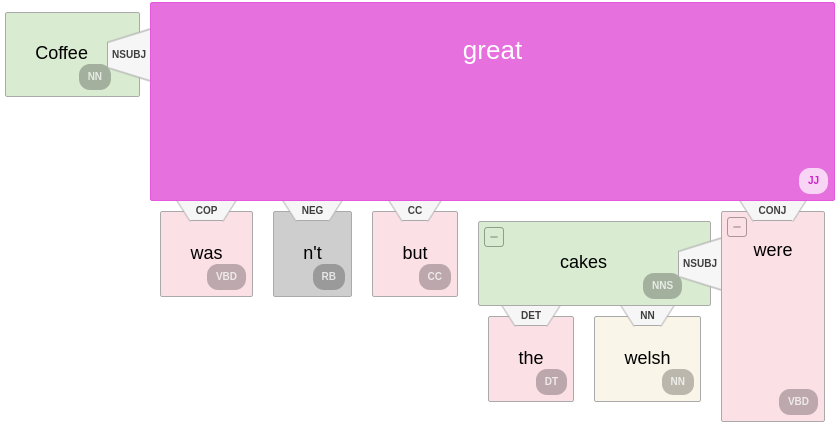
\includegraphics[scale=0.28]{images/lit_review/dependency_parse_tree.png}
    \caption{Dependency tree for the sentence `Coffee wasn't great but the welsh cakes were'. The labels within the arcs are dependency labels, and the labels within each box represents the POS tag for the given word. An arc from \textit{word A} to \textit{word B} indicates that \textit{B} is modifying \textit{A}, where \textit{A} is the head word. For example \textit{great} is the head word of \textit{coffee}. The tree was created using the AllenNLP demo, which used \citet{DBLP:conf/iclr/DozatM17} model.}
    \label{fig:lit_review_dependency_parse_tree}
\end{figure}

\section{Sentiment Analysis}
Sentiment analysis can be seen as a topic that contains multiple different tasks. These task tend to be related and often have different assumptions. In this section the different tasks within sentiment analysis  will be discussed and explicitly shown how they are related and towards the end of the section how they relate to the main topic of this thesis Target Dependent Sentiment Analysis (TDSA).

\subsection{Document Sentiment Analysis}
The most common sentiment analysis task is that of document level. The task here is given a document which is made up of multiple sentences, predict the sentiment. An example sample for this task can be seen in example \ref{example:lit_review_document_sentiment}. The first to apply a supervised machine learning algorithm to this problem was \citet{pang-etal-2002-thumbs}, where they applied several Machine Learning (ML) classifiers with Bag Of Words (BOW) as features to a new movie review dataset. This line of research of applying ML was further extended by \citet{pang-lee-2004-sentimental} who find that they can reduce the number of sentences by removing objective sentences in the document without significantly impacting and in some cases improving the overall accuracy of the classifier. \citet{mullen-collier-2004-sentiment} explored incorporating more semantic features into the BOW models such as the average sentiment values based on the unsupervised techniques of \citet{turney-2002-thumbs}. This approach of adding more semantic information into BOW models was further explored by \citet{whitelaw2005using} who created lexicon feature sets based around appraisal groups. Even though the use of semantic information had improved results \citep{whitelaw2005using}, the strong baseline performance of just using n-gram BOW features was further investigated by \citet{martineau2009delta} who showed that incorporating the class into the TFIDF weighting mechanism \citep{jones1972statistical} to create Delta TFIDF significantly improved results. However Delta TFIDF was only created to work with two classes\footnote{In the sentiment case this is the positive and negative classes.} and not shown to generalise to \textit{n} classes. However a future study by \citet{paltoglou-thelwall-2010-study} showed that further performance gains can be made to TFIDF based systems by using more enhanced weighting systems like BM25 \citep{robertson1995okapi}.

\begin{example}
\textit{a couple of criminals ( mario van peebles and loretta devine ) move into a rich family's house in hopes of conning them out of their jewels . however , someone else steals the jewels before they are able to get to them . writer mario van peebles delivers a clever script with several unexpected plot twists , but director mario van peebles undermines his own high points with haphazard camera work , editing and pacing . it felt as though the film should have been wrapping up at the hour mark , but alas there was still 35 more minutes to go . daniel baldwin ( i can't believe i'm about to type this ) gives the best performance in the film , outshining the other talented members of the cast .}
\caption{Negative document level sentiment example. Document ID \textit{cv435\_24355} taken from \citet{pang-etal-2002-thumbs} sentiment dataset.}
\label{example:lit_review_document_sentiment}
\end{example}

The supervised approaches that have been mentioned so far use a BOW approach, of which this form of vector representation is limited in what it can represent. BOW approaches that use n-gram word features can only learn what a word means within that \textit{n} window. For instance take \textit{n} to be 1 and 2\footnote{uni-gram and bi-gram features.} it would understand terms such as `very good' and `good' where both would be associated with positive sentiment, however if the statement was `not very good' then it would not capture the full sentiment as it would require all three words to know it's negated. One approach would be to have a very large value for \textit{n}, but this would create a very sparse vector representation which would not generalise well \citep{le2014distributed}. Thus the move away from BOW sparse vector representations to dense word representations was shown to be promising for sentiment analysis in \citet{maas-etal-2011-learning} work. However this work only found better performance than BOW when they combined the dense vectors with the BOW sparse vector. This first step into dense representation did show some promise as the representation can be learnt from unlabelled data, of which they found that results increased when more unlabelled data was used. These dense representations are very similar to what a traditional BOW model learns through it's weights within the model \citep{goldberg2017neural}\footnote{See section 2.5.}. The benefit of using the dense representations on the downstream task (sentiment analysis) is that a good representation of the vectors can be learnt from another unsupervised task from unlabelled data first\footnote{The task can also be supervised, but would required labelled data.}. Thus allowing the model to have prior knowledge of what words mean (semantically and syntactically \citep{mikolov2013efficient}) encoded into the vector representation before training the model, unlike the BOW representation which contains no prior knowledge. 

\citet{le2014distributed} showed for the first time how dense vector representations using a NN could surpass BOW representation of which \citet{wang-manning-2012-baselines} set a high baseline at the time for a BOW method. \citet{le2014distributed} created dense document/paragraph vector representations that in comparison to the prior word level versions \citep{maas-etal-2011-learning} could encode document size texts without averaging by learning to predict the next word within a small context window from the document, thus each document vector would be different unlike the word representations\footnote{Unless two or more documents are identical.}. \citet{johnson-zhang-2015-effective} showed that without any additional unlabelled data unlike \citet{le2014distributed} a Convolution NN (CNN) can outperform the BOW approach. The CNN can be seen as a NN approach to a BOW model where by the CNN has a set of user defined window sizes of which these window sizes are analogous to n-grams in a BOW model. The CNN differs from the BOW model as it can generalise to unknown n-gram sequences, as it learns how to combine representation from multiple word representations to create the n-gram representation, rather than in the BOW case where it learns what that entire n-gram means and disregards similarities between n-grams based on the words within the n-gram. Furthermore the CNN model does not have the sparsity problem that a BOW model has thus the window size (n-gram in BOW case) can be large e.g. \citet{johnson-zhang-2015-effective} found that having a window size of 2 and 3 to perform best\footnote{\citet{le2014distributed} has a good summary of the drawbacks of BOW vector representations.}. For a more complete overview of CNNs read chapter 13 of \citet{goldberg2017neural}.

None of the above methods including the NN approach take into account the word order of the whole document. One family of NN that explicitly encodes whole sequence of text in word order is the Recurrent NN (RNN). The RNN has several popular variants Long Short Term Memory (LSTM) and the Gated Recurrent Unit (GRU). \citet{dai2015semi} showed practically that LSTMs can be used for long sequence classification tasks such as document sentiment classification. Hierarchical \citep{zhang2015character} and dilated \citep{strubell-etal-2017-fast} CNN approaches have been created which can capture large contexts e.g. sentences rather n-grams, of which they have been shown successful in sentiment analysis \citep{conneau-etal-2017-deep}. Finally and more recently the transformer NN \citep{vaswani2017attention} approach which does not preserve word order like the RNN or CNN but rather treats the text more like a tree structure through attention mechanisms, where by each word learns to contextualise itself within the text (can be the whole text). The transformer success can be best seen through BERT \citep{devlin-etal-2019-bert} where the transformer architecture can be applied to task like document sentiment analysis \citep{sun2019fine}. For a good comparison of RNN, CNN, and transformer based models with respect to computational cost see section 4 of \citet{vaswani2017attention}. The majority of these more recent NN approaches have been tested on much larger sentiment datasets (100Ks samples) compared to the earlier work (2-25K samples). It has also been shown that for some of these NN approaches to work well they require extra data \citep{dai2015semi}. However as found in \citet{dai2015semi} that these NN approaches can make great use of unlabelled data through a language modelling objective. This technique of training on one or more datasets and/or tasks before then applying the model to the end task (in this case document sentiment analysis) is defined as transfer learning in this thesis \citep{ruder2019neural}\footnote{Chapter 3}.  Both \citet{howard-ruder-2018-universal} and \citet{sun2019fine} found that by pretraining (a type of transfer learning) on the unlabelled data can have large performance gains, making the models more sample efficient with respect to labelled/annotated data. All of the neural methods within this paragraph take into account large contexts of the document if not the whole document, of which none of the previous methods could effectively. In doing so the methods can overcome one the main challenges in document sentiment analysis that both \citet{turney-2002-thumbs} and \citet{pang-etal-2002-thumbs} found that the sentiment of the whole document is not the `sum of the parts' \citep{turney-2002-thumbs}. Whether the methods actually overcome this problem is unknown and has not be explored.


\citet{pang-etal-2002-thumbs} created the first English dataset of movie reviews (1.4K samples), which was later revised and increased in \citet{pang-lee-2004-sentimental} (2K samples), and then increased a lot further by \citet{maas-etal-2011-learning} (25K samples). The prior datasets all contained only 2 classes positive and negative of which these were based on the user's star rating that the movie review was given. \citet{zhang2015character} created four much larger datasets (\~600K - \~4M samples) that have come from Yelp\footnote{https://www.yelp.com/dataset} and Amazon reviews \citep{mcauley2015image} of which they contain between two and five classes where the classes are based around the user's star rating. This list of English datasets is not suppose to be exhaustive but is given as reference to popular and widely used datasets from the past and current literature.

In this literature section document sentiment analysis has been covered with respect to supervised methods and the associated popular English datasets. From the literature it is clear to see that the SOTA are NN based methods that require some form of transfer learning \citep{yang2019xlnet}. All of the methods also clearly point to one of the main challenges in document sentiment analysis is the size of the documents. This can be seen from early in the literature where  \citet{turney-2002-thumbs} state that the sentiment of the whole document is not the `sum of the parts'. This therefore means that the whole document needs to be understood in context to fully understand the sentiment which has been shown not possible with the BOW methods. Thus the move to NN approaches such as the LSTMs, heirahcical CNNs, and transformers to overcome this problem.


%The main difficulty in document sentiment analysis has been shown through it's length Further sentiment lexicons have been defined and numerous NN methods have been introduced. 

%So far the supervised methods within document sentiment analysis have been covered, from which it is clear to see that the SOTA are NN based and require some form of transfer learning \citep{yang2019xlnet}. All of the methods also clearly point to one of the main challenges in document sentiment analysis is the size of the documents. This can be seen from early in the literature where  \citet{turney-2002-thumbs} state that the sentiment of the whole document is not the `sum of the parts'. This therefore means that the whole document needs to be understood in context to fully understand the sentiment which has been shown not possible with the BOW methods. Thus the move to NN approaches such as the LSTMs, heirahcical CNNs, and transformers to overcome this problem.


%can be used to c encode some form of word order within 
%The use of dense vector representations stayed at the forefront to State Of The Art (SOTA) document sentiment classification. 

% created a much large movie review sentiment dataset \citet{maas-etal-2011-learning}
%who explored different information retrieval weighting mechanisms

%\citet{whitelaw2005using} Created a apprisal lexicon through using a list of words that were known to be part of the lexicon as `seed words' and then expanding that list through collocations, WordNet, and thesauri

%Incorporating 

%The first document sentiment dataset was by \citet{pang-etal-2002-thumbs}, which was then later enlarged by \citet{pang-lee-2004-sentimental}

%This novel Machine Learning (ML) work was conducted at the same time as \citet{turney-2002-thumbs} who applied an un-supervised approach to the same problem, both came across the same problem, which is that the sentiment of the review cannot be determined through `sum of it's parts' \citep{turney-2002-thumbs}\footnote{This is paraphrased for grammatical reasons, the actual quote is `sum of the parts'}. This problem is due to both works only using BOW (up to bi-grams) features within their methods, thus their features only take into account local context and limited linguistic knowledge (POS tags in \citet{turney-2002-thumbs}). This problem to some extent started to be alievated with the raise of more 

\section{Target Dependent Sentiment Analysis}
The holder within TDSA can be first related back to \citet{{wiebe-1990-identifying} where they first explain in multiple different circumstances who the holder of the sentiment\footnote{In the original work they never used sentiment rather subjectivity but the two are rather similar in these circumstances.} is and the difference between the holder and the target\footnote{In the original work they used the word `experiencer' rather than `target'}. In this work they also stated the importance of co-reference resolution\footnote{co-reference and anaphora resolution within this thesis are the same task.} with respect to finding the holder and how it can span over multiple sentences.

The first to state the importance of using Target Dependent (TD) over non-TD methods\footnote{Non-TD method is any method where given a text will return only one sentiment for that text, no matter if the text contains different sentiments for the targets within that text. An example of these non-TD methods would be document/sentence/tweet sentiment analysis.} for TDSA was \citet{jiang-etal-2011-target} where they find 40\% of samples\footnote{Out of a total of 100 samples.} to be mis-classified by the non-TD method due to it finding the overall sentiment of the sample rather than the sentiment for the target within the text.  